% ----------------------------------------------------------
\section{Pré-processamento dos dados}
% ----------------------------------------------------------

Prévio ao processo de calibração foi realizado um processo de Pré-processamento dos dados para reduzir ruído e quantidade de \textit{outliers}. Para isso os dados foram etiquetados seguindo alguns pontos dos procedimentos descritos por \textit{AQMesh}, Ottosen e Kumar \cite{Ottosen2019OutlierMeasurements} e o Guia para monitoramento da qualidade do ar o IMA \cite*{INSTITUTODEENERGIAEMEIOAMBIENTE2019QualidadeAr}. O pré-processamento foi realizado utilizando a linguagem de programação Python e \textit{Jupyter Notebooks}. A continuação detalham-se as etiquetas utilizadas, entre parênteses é colocado o nome da etiqueta utilizada dentro do código. Os Anexos XXX a XXX contêm o código desenvolvido em \textit{Jupyter Notebooks} para o processo de filtragem dos dados dos sensores.

\begin{itemize}
    \item Dados faltantes (\textit{MISSING}): Esta etiqueta representa amostras faltantes na amostragem dos dados.
    \item Estabilização (\textit{STABILIZ}): A estabilização é um período em que um sensor fornece dados não confiáveis por não estar em estado de equilíbrio. Uma vez que o sensor se estabilizar em seu ambiente após ter sido movido recentemente ou após ter sido instalado pela primeira vez, ele fornecerá dados utilizáveis. Este processo leva 2 dias para ser concluído para sensores eletroquímicos, não sendo necessário para o sensor de material particulado modelo OPC de Alphasense (Manual de procedimento de operação padrão AQMesh). Neste trabalho foi utilizado um período de 7 dias para garantir uma maior estabilidade do sensor.
    \item Dados acima do Limite Superior (\textit{GTUL}): Essa etiqueta está relacionada a valores que ultrapassam o limite superior do sensor. As especificações do fabricante ou valores conhecidos do poluente podem ser utilizados para definir esse limite. Por exemplo, o sensor Alphasense CO-B4 tem um limite de 1.000 ppm, equivalente a 1.000.000 ppb. Os valores que ultrapassaram esses limites para cada sensor foram removidos por serem indícios de alguma falha ou mal funcionamento do sistema de medição.
    \item Dados abaixo do Limite Inferior (\textit{LTLL}): Esta etiqueta sugere valores que estão abaixo da resolução do sensor e pode estar relacionada a possíveis valores negativos. A definição desse limite depende das especificações do sensor utilizado. O sistema de medição desenvolvido identifica valores faltantes ou NaN com o valor -9999.99. Por esse motivo, valores abaixo de -1000 ppb nos dados representam estas amostras depois de passar pelo processo de suavização.
    \item Dados com alteração do valor de linha base (\textit{REBASE}): Nas séries temporais dos sensores foram identificados alterações no valor de linha base das leituras. Observou-se também que nesses intervalos de variação da linha base a distribuição dos dados também estava alterada. Por esse motivo, os dados nesses intervalos foram marcados e removidos.
    \item Dados do quartil 99 \% (\textit{GTQTLE99}): Essa etiqueta está relacionada aos valores que se encontram no quartil 99 \% no histograma dos dados. Valores dentro desse intervalo foram etiquetados para remoção.
    \item Dados do quartil 1 \% (\textit{LTQTLE01}): Essa etiqueta está relacionada aos valores que se encontram no quartil 1 \% no histograma dos dados. Valores dentro desse intervalo foram etiquetados para remoção.
    \item Baixo número de amostras (\textit{LOWSAMPLES}): De acordo com o Guia de Monitoramento da Qualidade do Ar (IMA), pelo menos 3/4 das medições de uma hora devem ser válidas para o cálculo da média horária. No sistema desenvolvido, como o período de amostragem foi de 15 minutos, para uma média horária ser considerada válida, ela deve ser calculada por 3 ou 4 pontos.
    \item Transições abruptas nos dados (\textit{BADSPIKE}): Transições muito abruptas na série de dados também foram identificados. Para isso foram calculadas as derivadas das séries temporais e os valores comparados com o valor máximo das derivadas das séries temporais de referência. Valores de derivadas na série de dados acima desse valor máximo foram identificados como transições muito abruptas e etiquetados para remoção.
    \item Dados inválidos de temperatura \textit{INVALID\_ENV}: Aos dados de temperatura também foram aplicadas as etiquetas descritas anteriormente, com exceção de \textit{STABILIZ} e \textit{BADSPIKE}. Os valores de concentração de gás adquiridos no mesmo instante de algum dado inválido de temperatura foram marcados como \textit{INVALID\_ENV} para remoção.    
\end{itemize}

\subsection{Metodologia de preprocessamento das séries temporais}

Utilizando as etiquetas mencionadas anteriormente, foi aplicada uma metodologia de pré-processamento para remoção de ruído e outliers, conforme descrito a continuação.

\begin{enumerate}
    \item Suavização das curvas de dados com uma janela temporal de 1 hora: Primeiramente foi realizada a suavização das séries originais buscando reduzir o impacto de flutuações de curto prazo e realçar padrões de longo prazo, dado que os dados de referência encontram-se em períodos horários.
    \item Remoção do Período de Estabilização: Os primeiros 7 dias da série temporal foram desconsiderados. Essa decisão fundamenta-se na consideração de que nesse período inicial após a instalação o sensor encontra-se num estado de estabilização propenso a flutuações e ajustes. A remoção desses dados iniciais visa mitigar possíveis distorções na análise decorrentes desse período transitório.
    \item Remoção de valores fora de intervalo de medição: Em seguida, foram removidos os valores abaixo da resolução do sensor e acima do valor máximo do sensor. Tal procedimento tem por objetivo eliminar possíveis ruídos, registros muito extremos e falhas no sistema de medição que poderiam comprometer a integridade da série temporal.
    \item Remoção de valores com alterações na linha base: Para a detecção dos pontos em que a linha base das leituras sofreu alterações aplicou-se algoritmo \acrshort{pelt} \cite{Killick2012OptimalCost}. Este método foi aplicado por Ottosen e Kumar \cite{Ottosen2019OutlierMeasurements} para detectar mudanças abruptas na média e/ou na variância das séries temporais de sensores de gases. As leituras que apresentaram alterações na linha base foram desconsiderados já que nesses intervalos a distribuição dos dados também mudava e não apenas a linha base.
    \item Remoção de outliers por quartis: Consistiu na remoção dos quartis 1\% e 99\% dos dados agrupados por hora. Esse processo foi conduzido após a divisão dos dados em 24 grupos, representando cada hora do dia. Os quartis foram calculados individualmente dentro desses grupos, resultando em uma eliminação robusta de extremos estatísticos que poderiam introduzir viés na análise.
    \item Identificação e remoção de picos e outliers na derivada dos dados: Este passo envolveu a identificação e eliminação de picos na primeira derivada dos dados que excediam o valor máximo encontrado na derivada da série de dados de referência. Essa estratégia visa mitigar efeitos de variações abruptas, frequentemente associadas a falhas no sensor ou interferências externas.
    \item Re-amostragem para período de 1 hora: Este passo consistiu na re-amostragem dos dados para um período de 1 hora. Essa prática foi adotada para comparar e calibrar com os dados de referência que estão em períodos de uma hora.
    \item Remoção de médias com amostras insuficientes: Por fim, foram excluídas as médias de cada hora que não atingiram mais de 75\% de amostras válidas, equivalente a pelo menos 3 amostras por hora. Essa medida visa garantir a robustez estatística das médias horárias, excluindo intervalos com dados insuficientes para uma análise significativa.
\end{enumerate}

\begin{figure}[h]
    \centering
    \caption{Série temporal do sensor CO-B4}
    \begin{subfigure}{0.495\textwidth}
        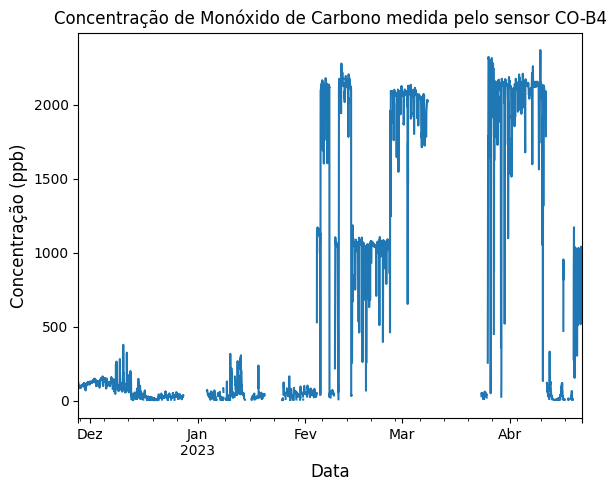
\includegraphics[width=\textwidth]{chapters/3-ANÁLISE DOS DADOS/Figuras/raw-co-b4.png}
        \caption{Série temporal do sensor depois de remover valores fora de intervalo}
        \label{fig:data-co-raw}
    \end{subfigure}
    \hfill
    \begin{subfigure}{0.495\textwidth}
        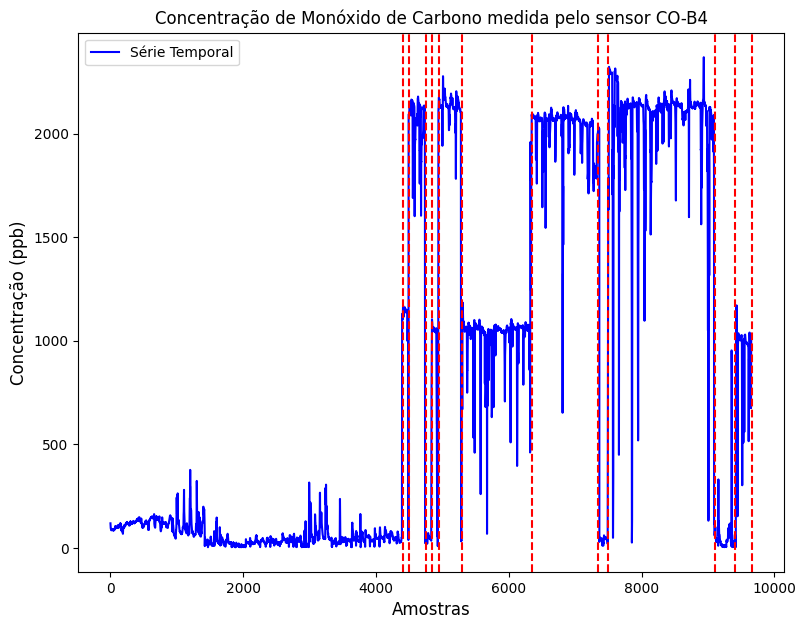
\includegraphics[width=\textwidth]{chapters/3-ANÁLISE DOS DADOS/Figuras/rebase-co-b4.png}
        \caption{Pontos de alteração da linha base detectados pelo algoritmo \acrshort{pelt}}
        \label{fig:data-rebase-co}
    \end{subfigure}
    \hfill
    \label{fig:data-co-raw-and-pelt}
    \fonte{Desenvolvido pelo autor (2023)}
\end{figure}

Uma vez pré-processados os dados dos sensores procedeu-se a realizar a calibração das leituras de \acrshort{co}, \acrshort{o3} e \acrshort{mp}, utilizando como referência os dados provenientes de uma estação de monitoramento de qualidade do ar. Foram explorados diferentes modelos multivariados para a calibração, i.e.: o Perceptron Multicamadas (MLP), Regressão Linear Multivariada (MLR), K Vizinhos mais Próximos (KNN) e as Florestas Aleatórias (RF). A escolha desses modelos baseou-se na capacidade de lidar com múltiplas variáveis simultaneamente, proporcionando uma adaptação mais eficaz às complexidades das relações entre os dados dos sensores e as condições ambientais de temperatura.

A calibração foi realizada em duas fases. Inicialmente, considerou-se apenas os dados do sensor em questão e a temperatura como variáveis de entrada. Para encontrar o modelo que melhor explicasse os dados foi realizada uma busca em \textit{grid} que combina diferentes parâmetros e variáveis de entrada e avalia cada modelo utilizando validações cruzadas com k = 3 Posteriormente, expandiu-se o escopo para incluir os dados de outros sensores disponíveis. Essa abordagem permitiu avaliar o impacto da inclusão de mais variáveis na precisão da calibração. A avaliação comparativa dos modelos de calibração foi realizada mediante métricas essenciais, incluindo o coeficiente de determinação (r2), o erro médio quadrático (RMSE) e o erro absoluto médio (MAE). A utilização de validações cruzadas proporciona uma análise mais robusta e imparcial do desempenho dos modelos.

A expectativa é que a implementação desses modelos de calibração aprimore significativamente a qualidade dos dados, fornecendo uma base sólida para análises subsequentes relacionadas à qualidade do ar. Os resultados desta pesquisa têm o potencial não apenas de beneficiar a precisão dos dados locais, mas também de contribuir para o desenvolvimento de metodologias aprimoradas de calibração em ambientes de monitoramento ambiental.